\documentclass[10pt]{article}
\usepackage[margin=.8in]{geometry}
\usepackage{booktabs,longtable,tabularx,graphicx,hyperref,amsmath}
\title{Original VERA: Result Reassessment and XD Confirmation Feasibility}
\author{Research report for Shrid Pant}\date{October 27, 2026}
\begin{document}\maketitle
\textbf{Decision: retain the original failed gate; recommend a separately preregistered CPU-only XD confirmation.} No XD performance experiment, feature download, GPU call, new annotation or training occurred in this reassessment. This recommendation responds to new human direction, not an automatic override of the original protocol.

\section{What the positive effect means}
On 290 UCF-Crime videos (1,111,808 frames), removing VERA's final Gaussian position weight raises worst-position ROC-AUC by \textbf{2.7211 percentage points}, with paired whole-video bootstrap 95\% interval \textbf{[1.3070,4.3714]}. The effect is positive under this resampling model and can be practically interesting. It does not meet the original requirement of at least 3 points; that gate remains \textbf{FAIL}. The interval includes effects both below and above 3 points, so it neither demonstrates the required effect size nor establishes that the true effect is below 3. Related/duplicate footage and five fixed counterfactual offsets limit inference.

The outcome is robustness to a final score-stage location intervention, not improved anomaly recognition or end-to-end video robustness. Pre-position scores and labels were circularly shifted together after refinement and smoothing, leaving evidence--label relationships fixed. The original final multiplier was then applied. Without that multiplier, shift invariance follows mathematically. No model or guiding question was changed.

\begin{center}\begin{tabular}{rrrr}\toprule
Offset (\%) & Original AUC (\%) & Without weight AUC (\%) & Original AP (\%)\\\midrule
0 &86.6071&85.6003&32.7449\\
20&84.6357&85.6003&26.8090\\
40&82.8792&85.6003&22.1868\\
60&84.2268&85.6003&25.5466\\
80&86.0362&85.6003&33.3768\\\bottomrule
\end{tabular}\end{center}
Without-weight AP is 28.7174\% at all offsets. Thus it loses 1.0068 AUC points and 4.0275 AP points on the original ordering; there is no uniform improvement.

\begin{center}\small\begin{tabular}{lrrrr}\toprule
Setting & Benefit (pp)&95\% interval (pp)&Original cost (pp)&Gate\\\midrule
15\% retrieval, all 290 &2.7211&[1.3070,4.3714]&1.0068&FAIL\\
15\%, exclude five &2.6995&[1.3460,4.3735]&1.1004&FAIL\\
10\%, all 290 &2.7581&[1.3477,4.3884]&1.0673&FAIL\\
10\%, exclude five &2.7336&[1.3767,4.3623]&1.1725&FAIL\\\bottomrule
\end{tabular}\end{center}
All four settings pass the positive-interval, spread and original-cost requirements but fail the 3-point benefit requirement. They are sensitivity analyses on overlapping data, not four independent replications. Each uses 1,000 paired whole-video bootstrap replicates.
\begin{figure}[ht]\centering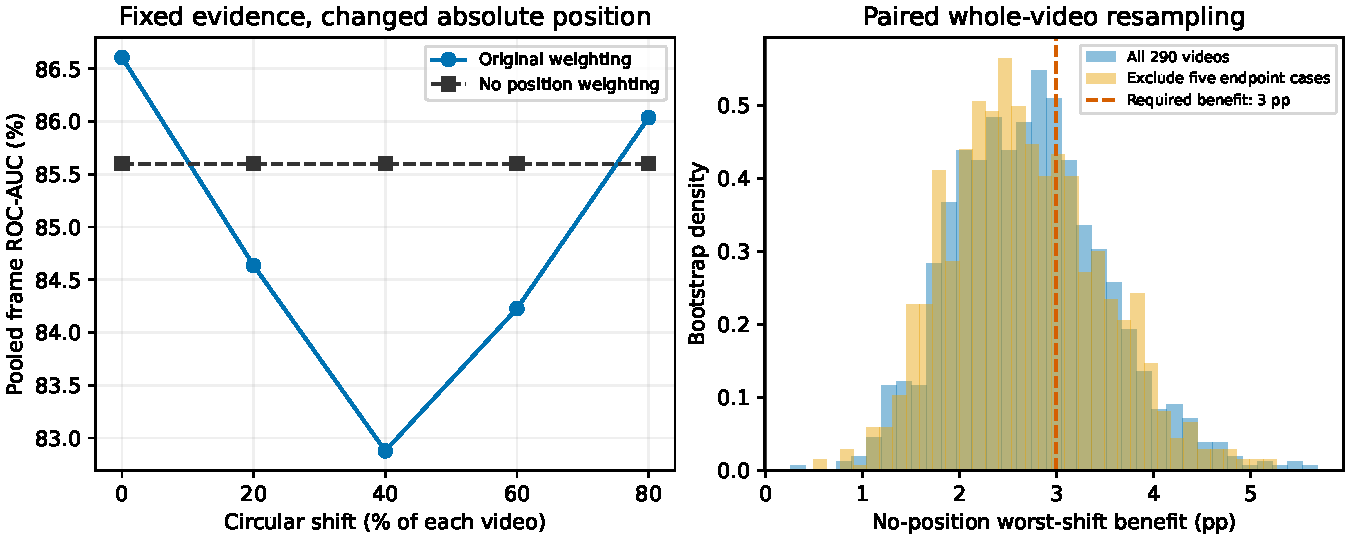
\includegraphics[width=\linewidth]{figures/position_audit.pdf}
\caption{Previously measured frozen UCF results; no new performance measurements in this reassessment.}
\end{figure}

\section{Chronology and why earlier directions stopped}
Times below use America/New\_York, EDT (UTC$-4$). Exact inference end times are derived from recorded start plus recorded wall duration where available. Commit times identify reporting/freeze events rather than inferred compute start times.
\small\begin{longtable}{p{2.65cm}p{3.1cm}p{9.0cm}}\toprule
When & Study & Result and limitation\\\midrule\endhead
Oct22 15:59--16:05 & Experiment01 & Single RoadAccidents127 reproduction: 99.4941\% within-video AUC, 15/15 validation. Not benchmark-wide AUC.\\
Oct22 20:13--20:30 & Experiment02 & 270 generation plus270 score calls. Accident singleton perturbations flipped0/8 for blur and grey; pedestrian singleton flips5/8 blur,8/8 grey. Local intervention sensitivity, not semantic faithfulness.\\
Oct23 14:10--Oct24 05:15 & Experiment03B & 199 original alerts/138 videos. Blur-ranked top-two grey replacement exceeded exact random-pair mean by15.1656pp [9.8599,20.6004]. This is alert removal, not accuracy gain.\\
Oct26 23:43:45 & 03B audit commit0e31840 & Original16/20 validator result preserved; amended validator20/20. BF16 tolerance, mask flags, black-frame no-op blur and duplicate-source cache contracts documented. No inference/result changes.\\
Oct27 00:32:31--00:34:01 & Temporal probe &40calls/8windows. Repeats8/8 identical; reverse/shuffle0/8 decision flips; repeated single frame2/8. Too small and unlabelled to support temporal correctness or learning.\\
Oct27 01:02--01:32 & UCA feasibility decisions &1,854videos/23,542captions available. Split overlap and caption incompleteness documented; absence of a caption is not falsehood. No caption-supervised training launched.\\
Oct27 12:18:53--12:21:04 & Abstention proxy &48calls/24inputs. Insufficient decisions1/12 annotation-included vs5/12 gaps; retained6/7 annotation-included original alerts. Gaps are not known negatives; accuracy unmeasured.\\
Oct27 13:26:49--13:29:59 & Selective explanations &72calls. Original12alerts; both modified prompts5. Manual JSON18/24 valid, all observations empty. Cited22/24 valid,17empty; four of five populated responses copied placeholders. No grounding benefit established.\\
Oct27 from13:32:11 & One prompt repair &Stopped at6calls when a response omitted final Output. No complete comparison; finish time unavailable. Preserved raw partial run; no retries or learning.\\
Oct27 14:17:32/14:24:07/14:30:38 & CPU position audit &Protocol freeze / final replay amendment / results commit. Successful replay22.257s; statistics206.368s. Absolute compute start not recorded; bounded by amendment and result commits. GateFAIL, positive measurable effect preserved.\\\bottomrule
\end{longtable}\normalsize

\section{Novelty reassessment: narrow and provisional}
VERA already reports no-position ablations (Table6 and AppendixB.4/Table17): 85.48\% without weighting versus86.55\% with it. CoReVAD also ablates the component. Removing it is not a new method. Sources: \url{https://arxiv.org/html/2412.01095v2}, \url{https://arxiv.org/html/2605.23116v1}.

Two additional primary sources narrow the broad audit claim: Song and Lee, \emph{Frame-Level Evaluation in Weakly Supervised Video Anomaly Detection Mostly Measures Video-Level Ranking}, audits released outputs, within-video permutation and pooled metrics across UCF/XD/ShanghaiTech (\url{https://arxiv.org/html/2608.21854v1}); Abdulaziz and Bondarev, \emph{Auditing Frame-Level AUC in Weakly Supervised Video Anomaly Detection: Granularity, Resolution, and Scene Bias}, compares evaluation granularities and paired-video uncertainty (\url{https://arxiv.org/html/2608.11985v2}). Neither inspected text establishes priority for our exact final-position replay; a targeted search failing to find it is not proof of novelty.

The defensible candidate is a reproducible, mechanism-specific measurement of the robustness--native-performance tradeoff caused by a recording-relative Gaussian prior, replicated on a second dataset and separated from pooled-ranking effects. It is presently a potential empirical contribution, not a novel detector or a demonstrated standalone publication. Do not claim temporal-localization auditing, paired bootstrapping or no-position removal as inventions.

\section{XD availability and the metric trap}
Metadata-only checks verified the1,471,961-byte public score ZIP (SHA256 \texttt{2564a0d1985dcd0643e7978db71bb3156cf8489858d3ff973a7fc40fc9598bc3}), ZIP CRCs and exact800-score/800-test-ID coverage. Anchor grids and final lengths match all800 metadata records; test records agree with the814-entry annotation source. All800 AP ground-truth arrays are binary and have the exact lengths produced by released AP trimming. The cohort spans2,335,801 metadata frames; maximum video length33,196frames. Feature metadata advertises652,318,723bytes; feature contents have \textbf{not} been downloaded or verified. Hashes identify observed bytes, not independent authenticity guarantees.

The released \texttt{compute\_auc\_XD\_Violence.py} applies final position weighting. The released \texttt{compute\_AP\_XD\_Violence.py} does not call it. Its sigmoid, one-decimal rounding, trimming and trapezoidal precision--recall area also differ from the AUC branch; that quantity must not be silently replaced by sklearn average precision. Both released scripts use smoothing15/sigma10 whereas the paper describes30/sigma30 for XD. These branches and discrepancies must be frozen and reproduced before evaluating any new claim. No-position removal cannot improve an official AP path that already omits position weighting.

\section{Recommended next experiment, not yet run}
A separately preregistered XD confirmation is worth a bounded CPU allocation because the UCF effect has a positive interval and the required released data are available. Freeze source hashes, all800 IDs, the same five offsets, no parameter tuning, paired-video resampling and resource bounds before feature download/performance. Verify all feature shapes, finiteness, norms and row alignment; reproduce the released AUC branch exactly. Abort on irreconcilable data/reconstruction errors; never substitute GPU features.

Primary reporting should retain the original3-point practical criterion and original-order cost ceiling1.5points, distinguishing a positive-effect replication (95\% lower bound above0) from meeting the practical criterion. Do not move the UCF goalpost or relabel its failed gate. Report the full fixed-offset curve and all tradeoffs. Reproduce the released AP branch separately; apply no fictitious weighting intervention to it. Predeclare within-video AUC as a secondary diagnostic, citing existing metric audits, with undefined single-class videos disclosed. Source-related XD clips may violate video-ID independence; predeclare a defensible source grouping/sensitivity before outcomes.

Suggested bound:30minutes CPU for reconstruction and30minutes for statistics, four BLAS threads, no GPU fallback and no automatic expansion. If XD does not corroborate a positive effect, preserve the UCF finding and close the cross-dataset claim. If it corroborates only a modest effect, report that outcome without asserting a novel algorithm. A positive replication strengthens the empirical case; it does not by itself resolve publication novelty.

\section{Audit trail}
Original UCF protocol819ba57, implementation3da8543, invocation fixbc7e03f, short-video replay correction3cce2c8, results99a6454 remain unchanged. All original result files and the original report are preserved. This additive reassessment and metadata-only checker are versioned in PR12: \url{https://github.com/shridpant/VERA/pull/12}. PR11 retains the prompt-study records and PR5 the03B repair. No merge.
\end{document}

